\documentclass{ximera}
\usepackage{sagetex}
%% handout
%% space
%% newpage
%% numbers
%% nooutcomes

%% You can put user macros here
%% However, you cannot make new environments

\graphicspath{{./}{module1Activity/}{module2Activity/}{module3Activity/}}

\usepackage{sagetex}
\usepackage{tikz}
\usepackage{hyperref}
\usepackage{tkz-euclide}
\usetkzobj{all}
\pgfplotsset{compat=1.7} % prevents compile error.

\tikzstyle geometryDiagrams=[ultra thick,color=blue!50!black]
 %% we can turn off input when making a master document

\outcome{}
\author{Darryl Chamberlain Jr.}
 
\title{Objective 2 - Graph Rational functions}

\begin{document}
\begin{abstract}
Convert between a rational function and its graph.
\end{abstract}
\maketitle

\href{https://cnx.org/contents/mwjClAV_@8.1:KNTP2r7D@13/Rational-Functions}{Link to section in online textbook.}

%%%%%%%%%%%%%%%%%%%%%
%%%  Objective 2  %%%
%%%%%%%%%%%%%%%%%%%%%

First, watch 
% UPDATE VIDEO LINK
\underline{\href{https://mediasite.video.ufl.edu/Mediasite/Play/4cff947227d54f71b32d175099114d3c1d}{this video}} 
to learn about what rational functions look like. We will work with two specific rational functions: $f(x) = \frac{1}{x}$ and $g(x)=\frac{1}{x^2}$. By using what we know about shifting and leading coefficients from Quadratics, Radicals, and Polynomials, we have two basic equations for rational functions: 

$$ f(x) = \frac{a}{x-h} + k $$

\[
\graph[rectangular]{f(x) = a/(x-h) + k, a=1, h=0, k=0, x=h, y=k}
\]

$$ g(x) = \frac{a}{(x-h)^2} + k $$

\[
\graph[rectangular]{f(x) = a/(x-h)^2 + k, a=1, h=0, k=0, x=h, y=k}
\]

Thinking back to the previous objective, our rational functions \textbf{are not defined at $x=h$.} So while $(h, k)$ acts like our vertex for quadratics, it is not actually a point on the graph! Check out the Desmos graphs to see how $a$, $h$, and $k$ affect the graphs of these two functions. 

We will focus on working from graphs to the equation. \textit{If you master this, you'll be able to work backwards and graph a radical function from the equation.} 

% Q1
\begin{question}
Write an equation of the function graphed below. Assume $a = 1$ or $a=-1$.

	\begin{center}
	    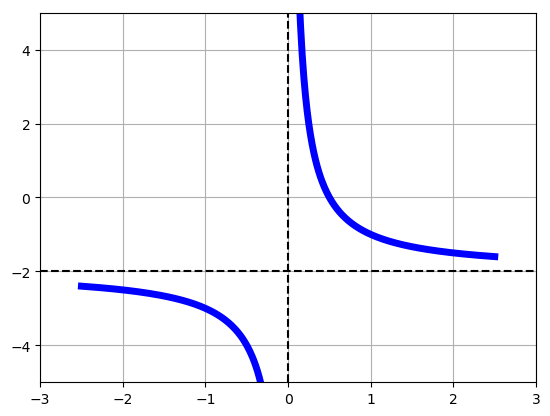
\includegraphics[width = 0.3\textwidth]{graphRationalQ1.png}
	\end{center}

$f(x) = \frac{\answer{1}}{(x - \answer{0})^{\answer{1}}} + \answer{-2}$

\begin{hint}
The leading coefficient is either $a=1$ or $a=-1$. Try going back to the Desmos graphs and switch between 1 and -1. For the other parts, what acts like the ``vertex" of the graph?
\end{hint}
\end{question}

% Q2
\begin{question}
Write an equation of the function graphed below. 

	\begin{center}
	    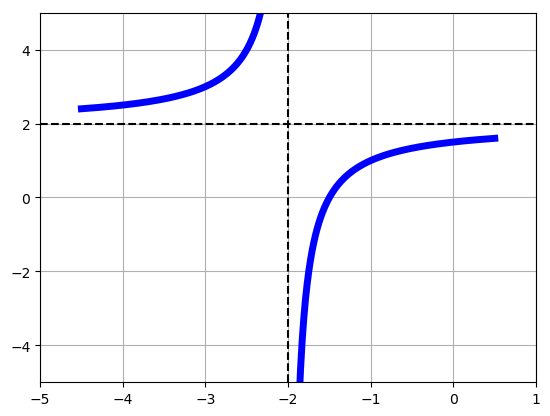
\includegraphics[width = 0.3\textwidth]{graphRationalQ2.png}
	\end{center}

$f(x) = \frac{\answer{-1}}{(x - \answer{-2})^{\answer{1}}} + \answer{2}$
\end{question}

% Q3
\begin{question}
Write an equation of the function graphed below. 

	\begin{center}
	    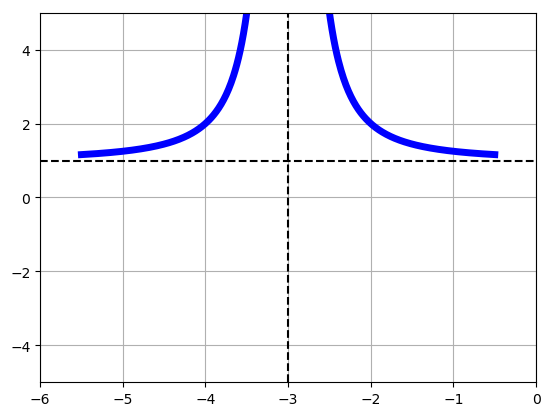
\includegraphics[width = 0.3\textwidth]{graphRationalQ3.png}
	\end{center}

$f(x) = \frac{\answer{1}}{(x - \answer{-3})^{\answer{2}}} + \answer{1}$
\end{question}

% Q4
\begin{question}
Write an equation of the function graphed below. 

	\begin{center}
	    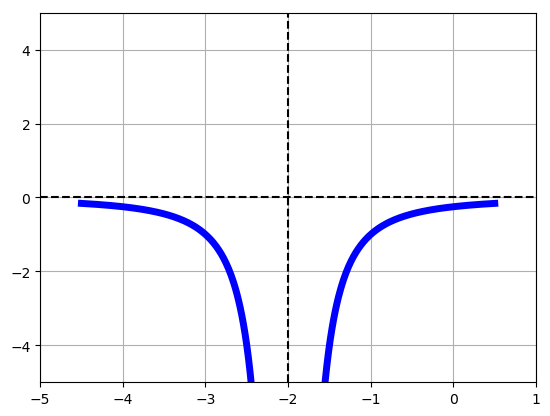
\includegraphics[width = 0.3\textwidth]{graphRationalQ4.png}
	\end{center}

$f(x) = \frac{\answer{-1}}{(x - \answer{-2})^{\answer{2}}} + \answer{0}$
\end{question}

% Q5
\begin{question}
Write an equation of the function graphed below. 

	\begin{center}
	    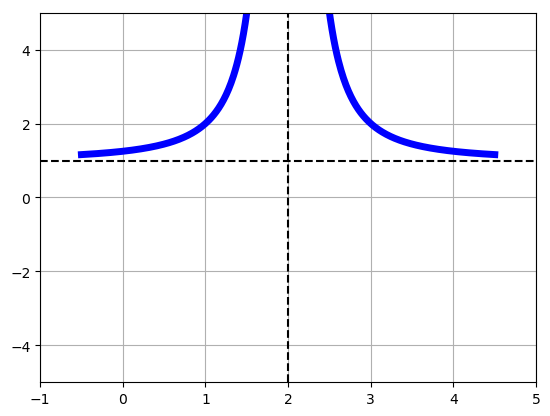
\includegraphics[width = 0.3\textwidth]{graphRationalQ5.png}
	\end{center}

$f(x) = \frac{\answer{1}}{(x - \answer{2})^{\answer{2}}} + \answer{1}$
\end{question}

% Q6
\begin{question}
Write an equation of the function graphed below. 

	\begin{center}
	    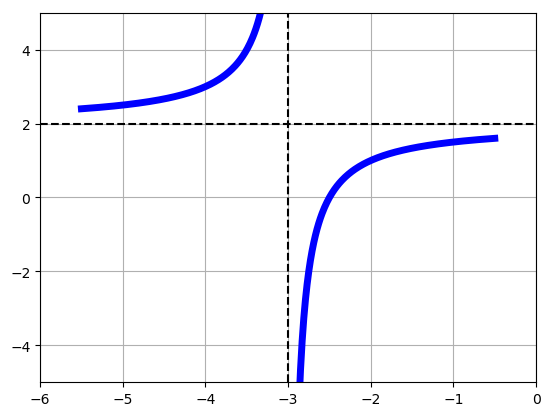
\includegraphics[width = 0.3\textwidth]{graphRationalQ6.png}
	\end{center}

$f(x) = \frac{\answer{-1}}{(x - \answer{-3})^{\answer{1}}} + \answer{2}$
\end{question}

% TAKEAWAY
\begin{question}
\textbf{Main takeaway:} Before looking, you should work through the previous problems. \textit{Have you finished working through the examples?} $\answer[format=string]{Yes}$
\begin{feedback}[correct]
The important components of a basic rational function are:
\begin{itemize}
	\item The vertical asymptote (\textit{vertical line where the function is not defined});
	\item Horizontal asymptote (\textit{horizontal line normally at $y=0$, shifted by $k$}); and
	\item The power of the denominator (\textit{1 has curves in opposite corners, 2 has curves side-by-side}).
\end{itemize}
\end{feedback}
\end{question}

\end{document}
